%=========================================================================================================
% capa

\setcounter{page}{0}

	
%CAPA
\onehalfspacing
\thispagestyle{empty}
\begin{center}
	{\textbf{UNIVERSIDADE FEDERAL DE ALFENAS}}\\
	\vspace{6cm}
    {\textbf{\teseauthorcap}}\\
	\vspace{6cm}
    {\textbf{\tesetitlecap}} 
	%\vspace{7cm}\\
	\vfill
	\textbf{ALFENAS     / MG\\
		2022}
\end{center}

% página em branco
%\newpage\null\thispagestyle{empty}\newpage

%=========================================================================================================
% folha de rosto

\newpage
%\section*{}
\vspace{-0.7cm}
\centerline{\textbf{\teseauthorcap}}
\vspace{3cm}
\begin{singlespace}
\begin{center}
\textbf{\tesetitlecap}
\end{center}
\end{singlespace}
\vspace{3cm}
\begin{flushright}
\begin{minipage}{12cm}
\begin{quote}
\begin{singlespace}
Dissertação apresentada à Universidade Federal de Alfenas, como parte dos requisitos para obtenção do título de Mestre em Estatística Aplicada e Biometria. Área de concentração: Estatística Aplicada e Biometria. Linha de pesquisa: Modelagem Estatística e Estatística Computacional. 

\vspace{0.1cm}
\noindent Orientadora: Prof. Dra. \teseorientador
\end{singlespace}
\end{quote}
\end{minipage}
\end{flushright}


\begin{center}
\begin{singlespace}
%\noindent Orientador\\
%\noindent Prof. Dr. \teseorientador

\vfill

\textbf{ALFENAS / MG\\ \teseyear}
\end{singlespace}
\end{center}

%=========================================================================================================
% ficha catalográfica
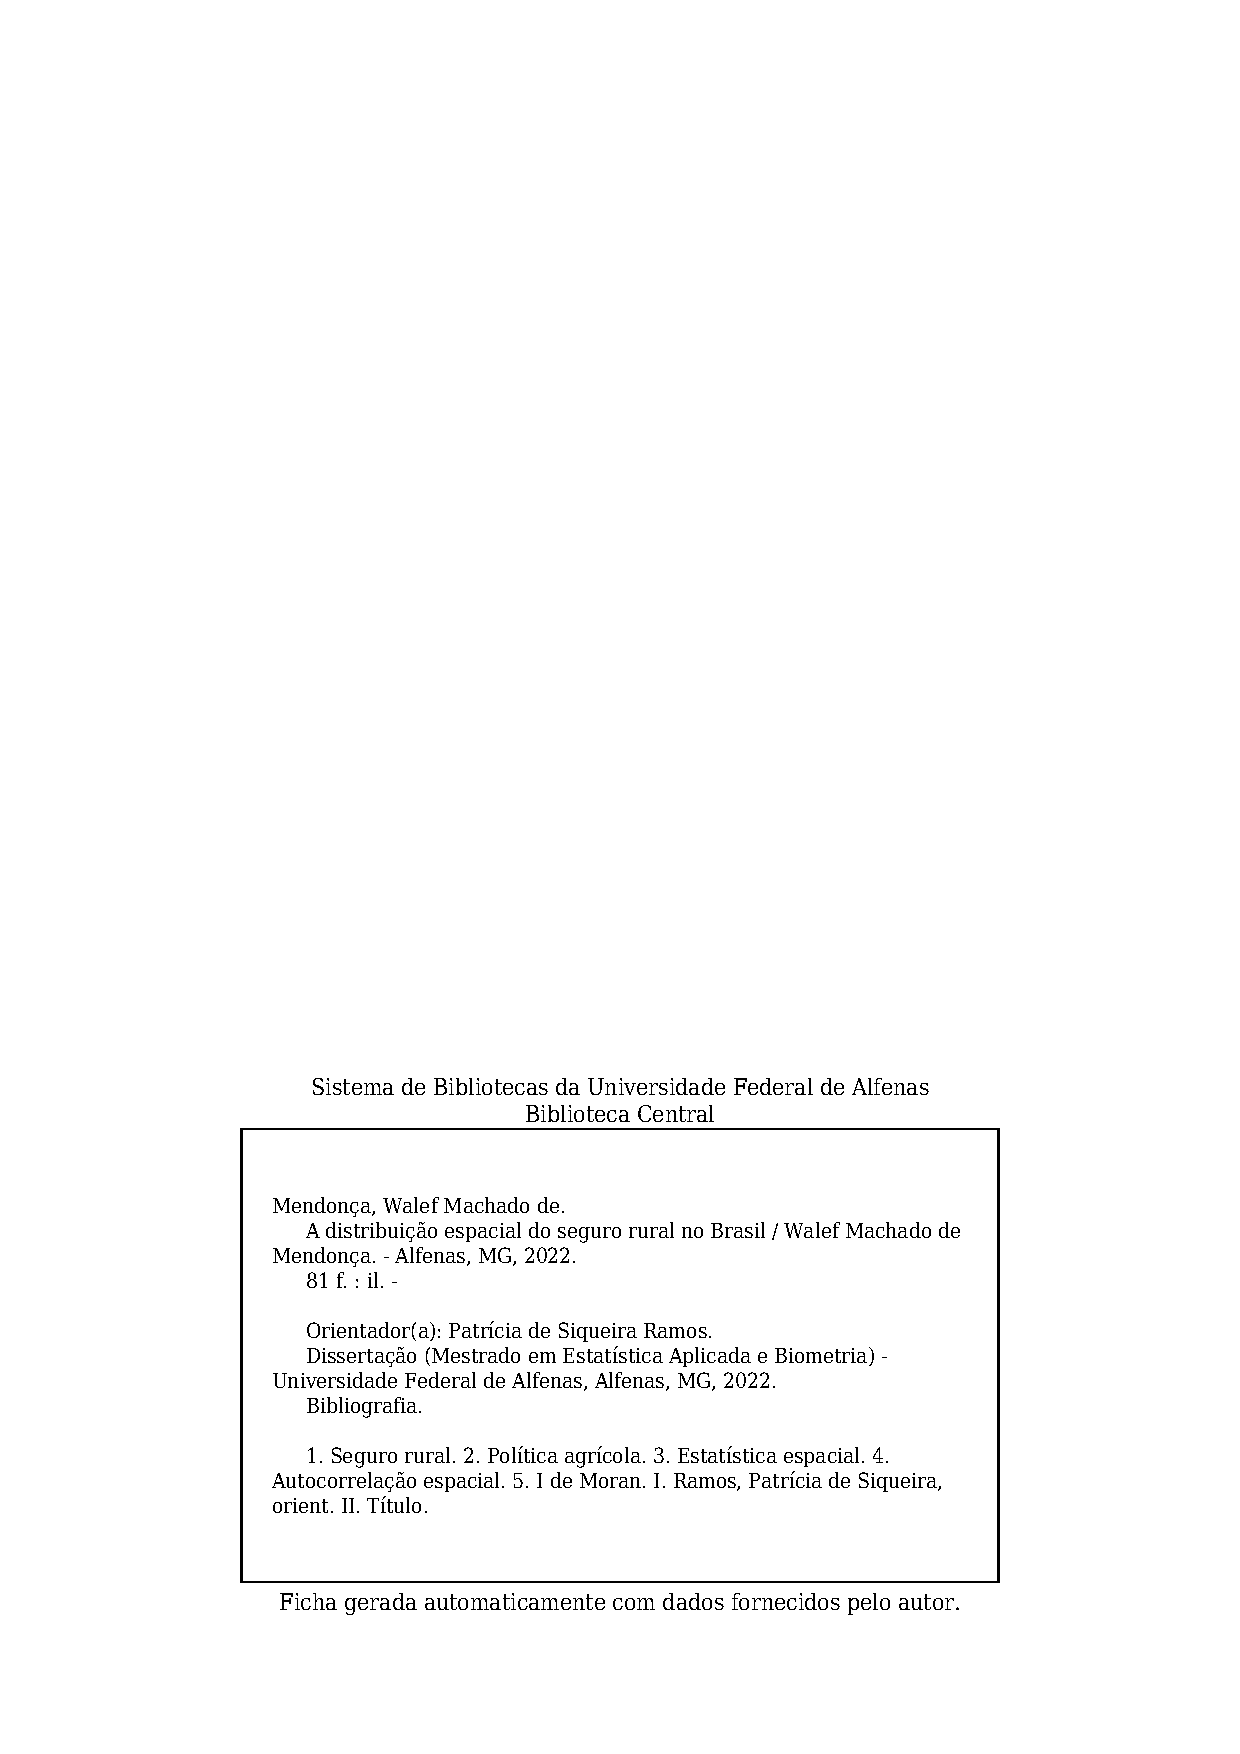
\includepdf[pages=1]{anexos/ficha_catalografica}

%\newpage
%\textcolor{white}{fantasma}

%\vfill
%\begin{center}
%\begin{singlespace}
%Dados Internacionais de Catalogação-na-Publicação (CIP) \\
%Sistema de Bibliotecas da Universidade Federal de Alfenas
%\vspace{-0.2cm}
%\end{singlespace}
%\end{center}
%\begin{center}
%\begin{boxedminipage}{12.8cm}
%\begin{singlespace}
%\begin{center}
%\hspace*{0.8cm}
%\begin{tabular}{p{11cm}}
%\vspace{0.5cm} \noindent{\teseauthorrev.}\\
%\hspace*{0.5cm} \tesetitle{} / \teseauthor.  -- Alfenas : UNIFAL, \teseyear.\\
%\hspace*{0.5cm} %\pageref{ultima} p. : il.
%\vspace{0.4cm}

%\hspace{0.5cm} Orientador: \teseorientador.\\
%\hspace{0.5cm} Dissertação (Mestrado em Estatística Aplicada e Biometria) -- Universidade Federal de Alfenas, \teseyear.\\
%\hspace{0.5cm} Bibliografia.

%\vspace{0.4cm}

%\hspace{0.8cm} .
%1. Análise espacial (Estatística). 2. Estatística agrícola. 3.
%Seguro rural. I. Ramos, Patrícia de Siqueira. II. Título. \\
%\multicolumn{1}{r}{}\\
%\multicolumn{1}{r}{}
%\end{tabular}
%\end{center}
%\end{singlespace}
%\end{boxedminipage}
%\vspace{0.2cm}
%\begin{singlespace}
%Ficha Catalográfica elaborada por -- \\
%Bibliotecária-Documentalista --
%\end{singlespace}
%\end{center}
%\pagebreak[4]

%=========================================================================================================
% página de aprovação
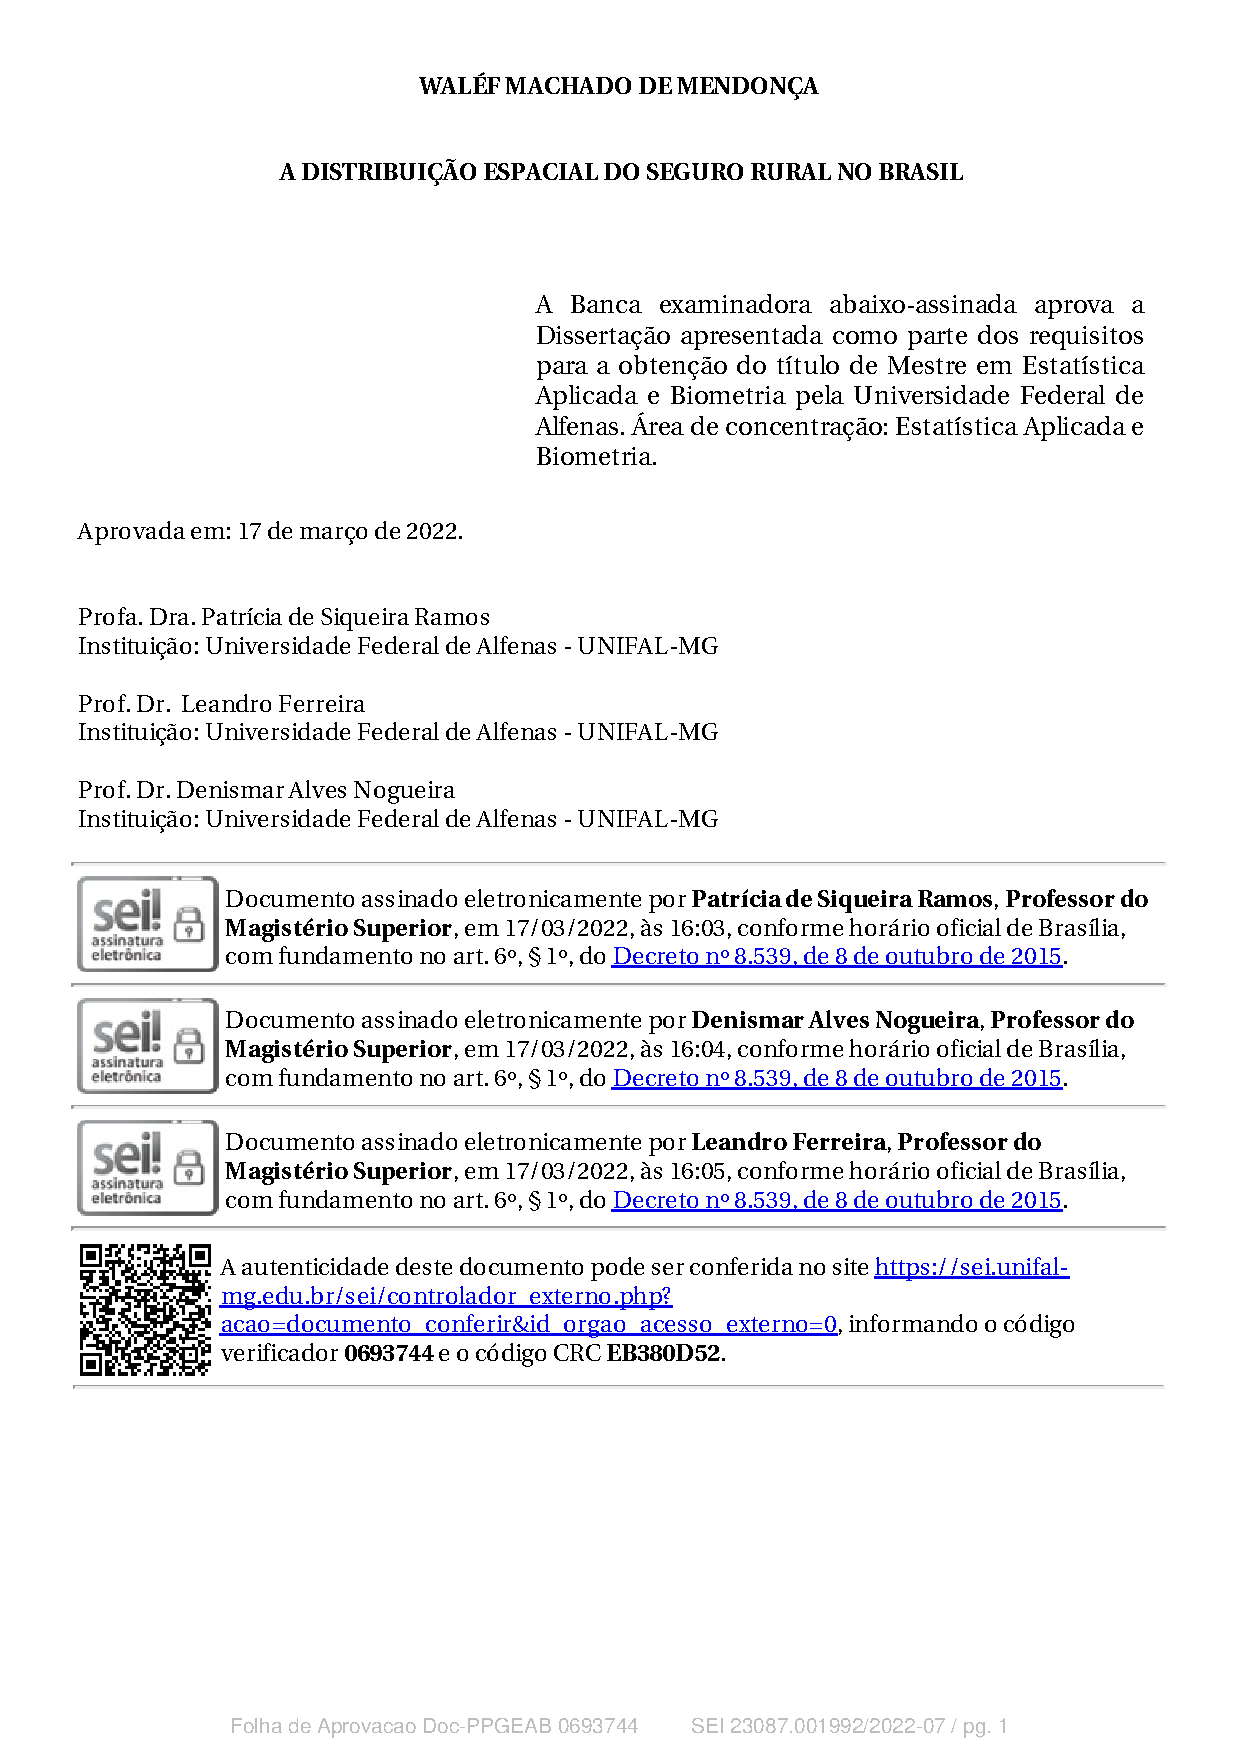
\includepdf[pages=1]{anexos/aprovacao_walef}

%\newpage
%\section*{}
%\vspace{-0.7cm} \centerline{\textbf{\teseauthorcap}}
%\vspace{1.4cm}
%\begin{singlespace}
%\begin{center}
%\textbf{\tesetitlecap}
%\end{center}
%\end{singlespace}
%\vspace{0.5cm}

%\begin{flushright}
%\begin{minipage}{9.6cm}
%\begin{quote}
%\begin{singlespace}
%A Banca examinadora abaixo-assinada, aprova a Dissertação apresentada como parte dos requisitos para obtenção do título de Mestre em Estatística Aplicada e Biometria pela Universidade Federal de Alfenas. Área de concentração: Estatística Aplicada e Biometria. Linha de pesquisa: Modelagem Estatística e Estatística Computacional.
%\end{singlespace}
%\end{quote}
%\end{minipage}
%\end{flushright}
%\vspace{1cm}

%\noindent\begin{tabular}{ll}
%Aprovado em XX de XXXX de 2022. \\
%\\
%\\
%Prof. Dra. \teseorientador & Assinatura:\\
%Instituição: Universidade Federal de Alfenas \\
%\\
%Prof. Dr. Leandro Ferreira & Assinatura:\\
%Instituição: Universidade Federal de Alfenas\\
%\\
%Prof. Dr. Denismar Alves Nogueira & Assinatura:\\
%Instituição: Universidade Federal de Alfenas\\
%\\


%\end{tabular}
%\begin{center}
%\begin{singlespace}
%%\vspace{0.8cm}
%\centerline{Prof. Dra. \teseorientador}
%\centerline{Orientadora}
%\vfill
%{\textbf{ALFENAS - MG\\ \teseyear}}
%\end{singlespace}
%\end{center}

% página em branco
%\newpage\null\thispagestyle{empty}\newpage

%=========================================================================================================
% dedicatória
\section*{}
\vspace{20cm}
\begin{flushright}

\textit{
\hspace{8cm} Aos meus pais, Adelvando e Dionísia, e a
\hspace{7cm} minha tia Cleonice, por todo amor e cuidado.}
\hspace{15cm}\textbf{Dedico este trabalho a vocês.}
\end{flushright}

% página em branco
%\newpage\null\thispagestyle{empty}\newpage

%===============================================================================
% agradecimentos

\newpage
\begin{center}
\textbf{AGRADECIMENTOS}
\end{center}
\vspace{0.5cm}

A maior parte dos ensinamentos que eu adquiri não foram através da análise de dados, sentado na frente de um computador, ou lendo pesquisas acadêmicas -- apesar de ter feito muito isso --, mas sim através da convivência com pessoas fantásticas cujas contribuições merecem algumas palavras de agradecimento. 

Nestes quase $7$ anos de graduação e pós-graduação na Universidade Federal de Alfenas eu tive o privilégio de estudar e trabalhar com pessoas que transformaram minha maneira de compreender o mundo e tornaram minha vida muito mais rica. 

Sou muito grato a todos os bons professores que pude conhecer na Unifal, tanto na graduação quanto no mestrado. Pude aprender um com cada um deles. 

Agradeço especialmente aos professores e amigos Patrícia Ramos e Lincoln Frias que, pacientemente, me acompanharam e apoiaram desde o início da graduação e que nunca deixarão de ser uma grande fonte inspiração em minha vida.

Agradeço também a generosidade dos professores Leandro Ferreira e Denismar Alves Nogueira. Os comentários e sugestões realizados durante o exame de qualificação e durante a defesa da dissertação contribuíram de forma decisiva para lapidar e direcionar o sentido do trabalho, além de proporcionarem reflexões para trabalhos futuros. 

Agradeço aos amigos que fiz na Unifal: Alice Duarte, Iris Rodrigues, Matheus Saraiva, Marcos Taroco, Poliana Benelli e Taylor Fidelis. O apoio dessas pessoas marcou profundamente minha formação intelectual e as minhas percepções com relação aos desafios da vida acadêmica. 

Sou muito grato também a todos os colegas que pude conhecer durante o mestrado. Agradeço especialmente o Giovani Festa e a Rafaela Gomes que tanto contribuíram para o meu aprendizado durante esses últimos dois anos. 

Não poderia deixar de agradecer também o constante apoio dos meus amigos Francisco Domingueti, Marcio Aloisio e Suzane Petruci. Nestes anos, que reforçaram a importância da proximidade espacial em todos os nossos relacionamentos, a presença dessas pessoas formaram os alicerces mais decisivos, através do apoio, compreensão, e orientações em todos os sentidos da minha vida.

O presente trabalho foi realizado com apoio da Coordenação de Aperfeiçoamento de Pessoal de Nível Superior – Brasil (CAPES) – Código de Financiamento 001

%===============================================================================
% epigrafe

\newpage
\section*{}
\vspace{16cm}


 
\setlength{\epigraphrule}{0pt}
\epigraph{
``Humans are good at discerning subtle patterns that are really there, but equally so at imagining them when they altogether absent.''}{Carl Sagan (1985)}

\setlength{\epigraphrule}{0pt}
\epigraph{
``In the face of ambiguity, refuse the temptation to guess''}{Tim Peters (2004)}


% página em branco
%\newpage\null\thispagestyle{empty}\newpage

%===============================================================================
